%Notes by Harsh Mistry 
%Econ 301
%Based on Template From  https://www.cs.cmu.edu/~ggordon/10725-F12/template.tex

\documentclass[twoside]{article}
\setlength{\oddsidemargin}{0.25 in}
\setlength{\evensidemargin}{-0.25 in}
\setlength{\topmargin}{-0.6 in}
\setlength{\textwidth}{6.5 in}
\setlength{\textheight}{8.5 in}
\setlength{\headsep}{0.75 in}
\setlength{\parindent}{0 in}
\setlength{\parskip}{0.1 in}
\usepackage{amsmath,amsfonts,graphicx, color}
\newcounter{lecnum}
\renewcommand{\thepage}{\thelecnum-\arabic{page}}
\renewcommand{\thesection}{\thelecnum.\arabic{section}}
\renewcommand{\theequation}{\thelecnum.\arabic{equation}}
\renewcommand{\thefigure}{\thelecnum.\arabic{figure}}
\renewcommand{\thetable}{\thelecnum.\arabic{table}}
\newcommand{\lecture}[4]{
   \pagestyle{myheadings}
   \thispagestyle{plain}
   \newpage
   \setcounter{lecnum}{#1}
   \setcounter{page}{1}
   
   
%Info Box 
   \begin{center}
   \framebox{
      \vbox{\vspace{2mm}
    \hbox to 6.28in { {\bf Econ 301 - Microeconomic Theory 2
	\hfill Winter 2018} }
       \vspace{4mm}
       \hbox to 6.28in { {\Large \hfill Lecture #1: #2  \hfill} }
       \vspace{2mm}
       \hbox to 6.28in { {\it Lecturer: #3 \hfill Notes By: #4} }
      \vspace{2mm}}
   }
   \end{center}
   
   \markboth{Lecture #1: #2}{Lecture #1: #2}



 
}

\renewcommand{\cite}[1]{[#1]}
\def\beginrefs{\begin{list}%
        {[\arabic{equation}]}{\usecounter{equation}
         \setlength{\leftmargin}{2.0truecm}\setlength{\labelsep}{0.4truecm}%
         \setlength{\labelwidth}{1.6truecm}}}
\def\endrefs{\end{list}}
\def\bibentry#1{\item[\hbox{[#1]}]}

\newcommand{\fig}[3]{
			\vspace{#2}
			\begin{center}
			Figure \thelecnum.#1:~#3
			\end{center}
	}
	
	\graphicspath{ {images/} }

\newtheorem{theorem}{Theorem}[lecnum]
\newtheorem{lemma}[theorem]{Lemma}
\newtheorem{ex}[theorem]{Example}
\newtheorem{proposition}[theorem]{Proposition}
\newtheorem{claim}[theorem]{Claim}
\newtheorem{corollary}[theorem]{Corollary}
\newtheorem{definition}[theorem]{Definition}
\newenvironment{proof}{{\bf Proof:}}{\hfill\rule{2mm}{2mm}}
\newcommand\E{\mathbb{E}}


%Start of Document 
\begin{document}

\lecture{6}{January 22, 2018}{Jean Guillaume Forand}{Harsh Mistry}
\section{Consumer Choice Continued}

\subsection{Optimal consumer choice}
\begin{center}
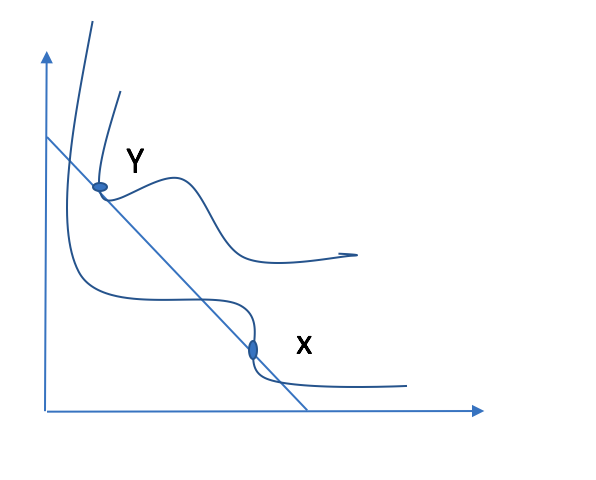
\includegraphics[scale=0.4]{11}
\end{center}
\begin{itemize}
\item FOC \((L1) - (L\lambda)\) are only \underline{necessary} for \(x^*\) to be optimal. (i.e any solution \(x^*\) to (PE) must be a solution to  \((L1) - (L\lambda)\) but some solutions to   \((L1) - (L\lambda)\) are not solutions to (PE) )
\item Need sufficient or second order conditions that guarantee that solutions to  \((L1) - (L\lambda)\) are also solutions to (PE)
\item Result if the consumers preferences are monotone and convex then any solution to  \((L1) - (L\lambda)\) must be a solution to (PE)
\end{itemize}

\begin{ex} Suppose \(U(x_1, x_2) = \sqrt{x_1} + x_2\) and solve for \(\sqrt{x} + x_2 = c\)
\begin{center}
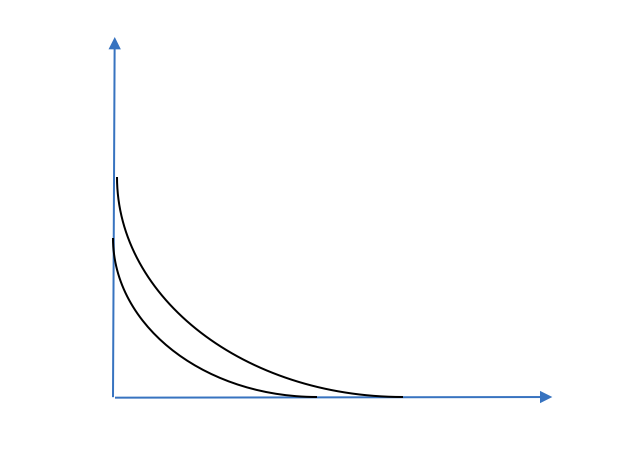
\includegraphics[scale=0.4]{10}
\end{center}
\begin{enumerate}
\item Consumer UMP 
\[\text{max}_{x_1, x_2 \geq 0} \hspace{0.2cm} \sqrt{x_1} + x_2  \text{ s.t } \hspace{0.2cm} p_1 x_1 + p_2x_2  \leq m \]
\item Preferences are monotone if \(x_1 > y_1\) and \(x_2 > y_2\) 
\[\begin{aligned}
U(x_1, x_2) & = \sqrt{x_1} + x_2 \\
&  > \sqrt{y} + y_2 \\
& = U(y_1, y_2) \implies x \succ y 
\end{aligned}\]
Therefore, budget constraint holds as an equality at any solution to UMP 
\item Lagrangian
\[L(x_1, x_2, \lambda) = \sqrt{x_1} + x_2 + \lambda [ m - p_1 x_1 - p_2 x_2 ]\]
\item Any solution to UMP such that \(x_1^* , x_2^* \neq 0\) must solve FOC (First Order Conditions) 
\[ \frac{d}{dx_1 } L(x_1, x_2, \lambda) = \frac{1}{2 \sqrt{x}} - \lambda p_1 = 0 \hspace{0.2cm} (L1) \]
\[\frac{d}{dx_2} L(x_1, x_2, \lambda)  = 1 - \lambda p_2 = 0 \hspace{0.2cm} L(2)\]
\[\frac{d}{d\lambda} L(x_1, x_2, \lambda)  = m - p_1 x_2^* - p_2x_2^* = 0 \hspace*{0.2cm} (L\lambda)\]
Divide \((L1)\) by \((L2)\)
\[\begin{aligned}
\frac{1}{2 \sqrt{x_1}} = \frac{p_1}{p_2}\\
x_1^* = \frac{1}{4} ( \frac{p_2}{p_1})^2    \hspace{0.2cm} (\star) 
\end{aligned}\]
Substitute \((\star)\) into \(L(\lambda)\) : 
\[x_2^* = \frac{m}{p_2} - \frac{1}{4} \frac{p_2}{p_1}\]
There is a condition though. \((L1) - (L\lambda)\) only has a solution if \(\frac{m}{p_2} > \frac{1}{4} \frac{p_2}{p_1}\)
\item At a corner solution with \(x_1^* = 0 \), necessary condition 
\[\frac{\frac{d}{dx_1} U(0, m/p_2)}{\frac{d}{dx_2} U(0, m/p_2)} \leq \frac{p_1}{p2}\]
Unfortunately 
\[\lim_{x\rightarrow \infty} \frac{\frac{1}{2\sqrt{x}}}{1}  = \infty\]
This inequality is never satisfied, so the equation never holds.

Therefore, at \(x_1 = 0\), teh slope of the IC will never be greater than the budget line

\item At corner solution with \(x_2^* = 0\), necessary condition 
\[\frac{\frac{d}{dx_1} U(m/p_1, 0)}{\frac{d}{dx_2} U(m/p_1, 0)} \geq \frac{p_1}{p2}\]
So, 
\[\frac{\frac{1}{2\sqrt{m / p_1 }}}{1} \geq \frac{p_1}{p_2} \implies \frac{m}{p_2} \leq \frac{1}{4} \frac{p_1}{p_2}]\]
\item Consumer preferences are convec so that any solution to necessary conditions  must be solution to UMP
\item Demand function 
\[(x_1(p_1 m), x_2 (p_2m)) = \begin{cases} 
\left( \frac{1}{4} (\frac{m}{p_2})^2 , \frac{m}{p_2} - \frac{1}{4} \frac{p_2}{p_1}\right) & \text { if  } 
\frac{m}{p_2} > \frac{1}{4} \frac{p_2}{p_1}\\
\left(  \frac{m}{p_2}, 0 \right) & \text { if    } \frac{m}{p_2} \leq \frac{1}{4} \frac{p_2}{p_1}\end{cases}\]
\end{enumerate}
\end{ex}

\begin{itemize}
\item If consumers utility function is not differentiable, then the Lagrangian does not apply 
\end{itemize}

\begin{ex} Consider perfect compliments where \(U(x_1, x_2) = min \{x_1, x_2\}\)
\begin{center}
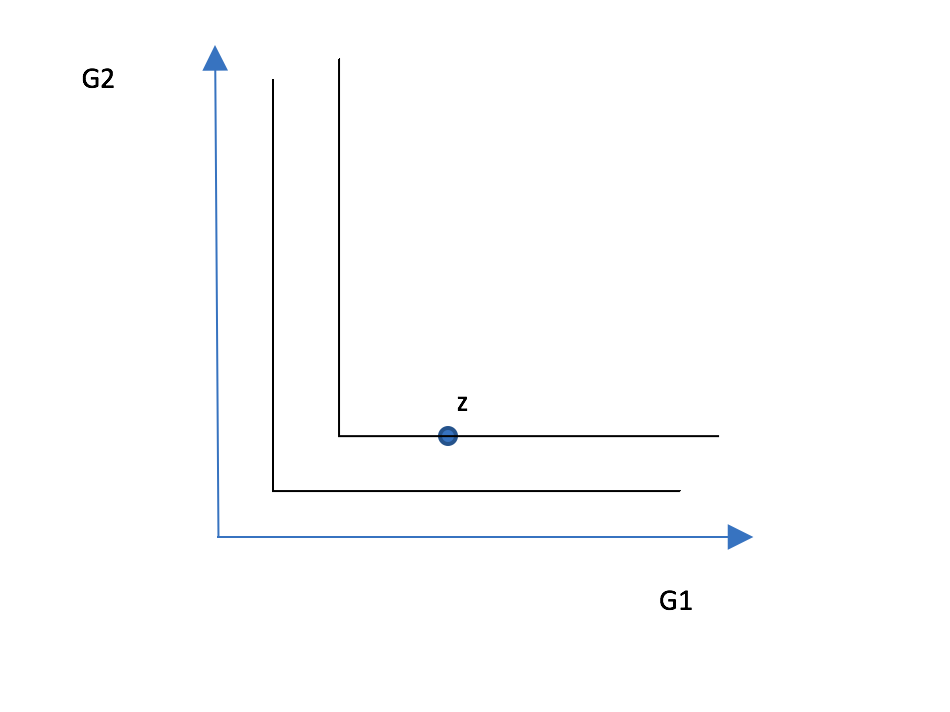
\includegraphics[scale=0.3]{6}
\end{center}
\begin{enumerate}
\item Consumers UMP 
\[\text{max}_{x_1, x_2 \geq 0} min\{x_1, x_2\} \hspace{0.2cm} \text{ such that } p_1x_1 + p_2x_2 \leq m \]
\item Consumer preferences are monotone. Let \(x_1 > y_1\) and \(x_2 > y_2\)
\[\begin{aligned}
U(x_1, x_2) & = min \{x_1, x_2\} \\
& > min  \{y_1, y_2\} \\
& = U(y_1, y_2) 
\end{aligned}\]
Therefore, budget constraint holds as an equality at any solution to UMP 
\item Any optimal bundle \(x^*\) must be such that \(x_1^* = x_2^*\). (I.e any bundle with \(x_1 > x_2\) is worse than bundles \(\left( \frac{m}{p_1 + p_2} + \frac{m}{p_1 + p_2} \right) \)
\item Demand Function
\[(x_1 (p_1m), x_2 (p_2 m) ) = \left(\frac{m}{p_1 + p_2} , \frac{m}{p_1 + p_2}  \right)\]
\end{enumerate}
\end{ex}

\end{document}





